\documentclass[12pt]{article}
\usepackage{lgrind}
\usepackage{fullpage}
\usepackage{graphicx}

\author{Bo Shi}
\title{6.111 Lab 3 Report \\ Digital Filter}
\date{October 13, 2004}


\begin{document}

\maketitle

\begin{abstract}
A digital filter that allows selection between all--pass, high--pass, box--car,
and exponential filters for an analog signal.
\end{abstract}

\newpage
% \pagenumbering{arabic}
% \setcounter{page}{1}
\section{Introduction}
	\subsection{High Level Design}
	In the steady state, 16 samples from the A/D chip are stored in RAM and
	the output is the convolution of the input signal with 4 possible impulse
	responses: all--pass, high--pass, box--car, and exponential.  The impulse
	responses are stored in ROM.

	The digital filter is implemented on an Altera Flex 10K10 FPGA clocked
	using a crystal oscillator running at 1.8472 Mhz.  For a sample rate of
	20 khz, this means that 92 clock cycles are available for sampling and
	convolution.  Sampling and convolution are the tasks which take the
	longest time.  This implementation samples and convolves in parallel.
	Sampling takes considerably less time than convolution.  Convolution is
	completed in approximately 64 clock cycles.

	The top level structure is shown in the block diagram.  The controller,
	A/D chip, and D/A chip are located on a 8-bit bidirectional bus.  A/D
	input is routed to RAM by the IO module.  The arithmetic unit responsible
	for convolution takes signal data and impulse response data from the RAM
	and ROM and routes the convolution signal back to the IO module.  There
	are three user inputs to the system, one of which is synchronized.  These
	are the reset (\texttt{rst}), ROM select (\texttt{romsel[1:0]}), and filter
	select (\texttt{fsel[1:0]}) signals.  The filter select chooses which 8
	bits of the 20-bit convolution output will be sent to the D/A buffer.  The
	latter two signals should be grounded or sourced, hence they are not
	synchronized.

	% \begin{table}
	% \centering
	% 	\begin{tabular}{|c|c|c|c|c|c|c|}
	% 	\hline
	% 	Bit 6 & Bit 5 & Bit 4 & Bit 3 & Bit 2 & Bit 1 & Bit 0 \\ \hline
	% 	Main Red & Main Yellow & Main Green & Side Red & Side Yellow & Side Green & Walk \\ \hline
	% 	\end{tabular}
	% \caption{Output Setup}
	% \label{tbl:output}
	% \end{table}
	

\section{Module Description}
	\subsection{IO Module}
	The IO module contains two buffers which store A/D input and convolution
	data.  The A/D minor FSM writes to the A/D buffer which holds samples until
	the RAM is ready.  The D/A buffer stores the results of the arithmetic unit
	until the D/A chip is ready to latch new values.  Since the D/A chip accepts
	data in unsigned format, the 2's complement results of the arithmetic unit
	are converted to unsigned binary values before being stored in the buffer.

	\subsection{Control FSM}
	The major FSM (Figure ~\ref{fig:majorfsm}) is responsible for sending data
	to the D/A chip and storing data received from the A/D chip to RAM.  In
	addition, it is responsible for delegating A/D chip control and convolution
	to two minor FSM's.

	\begin{figure}[ht]
	\centering
	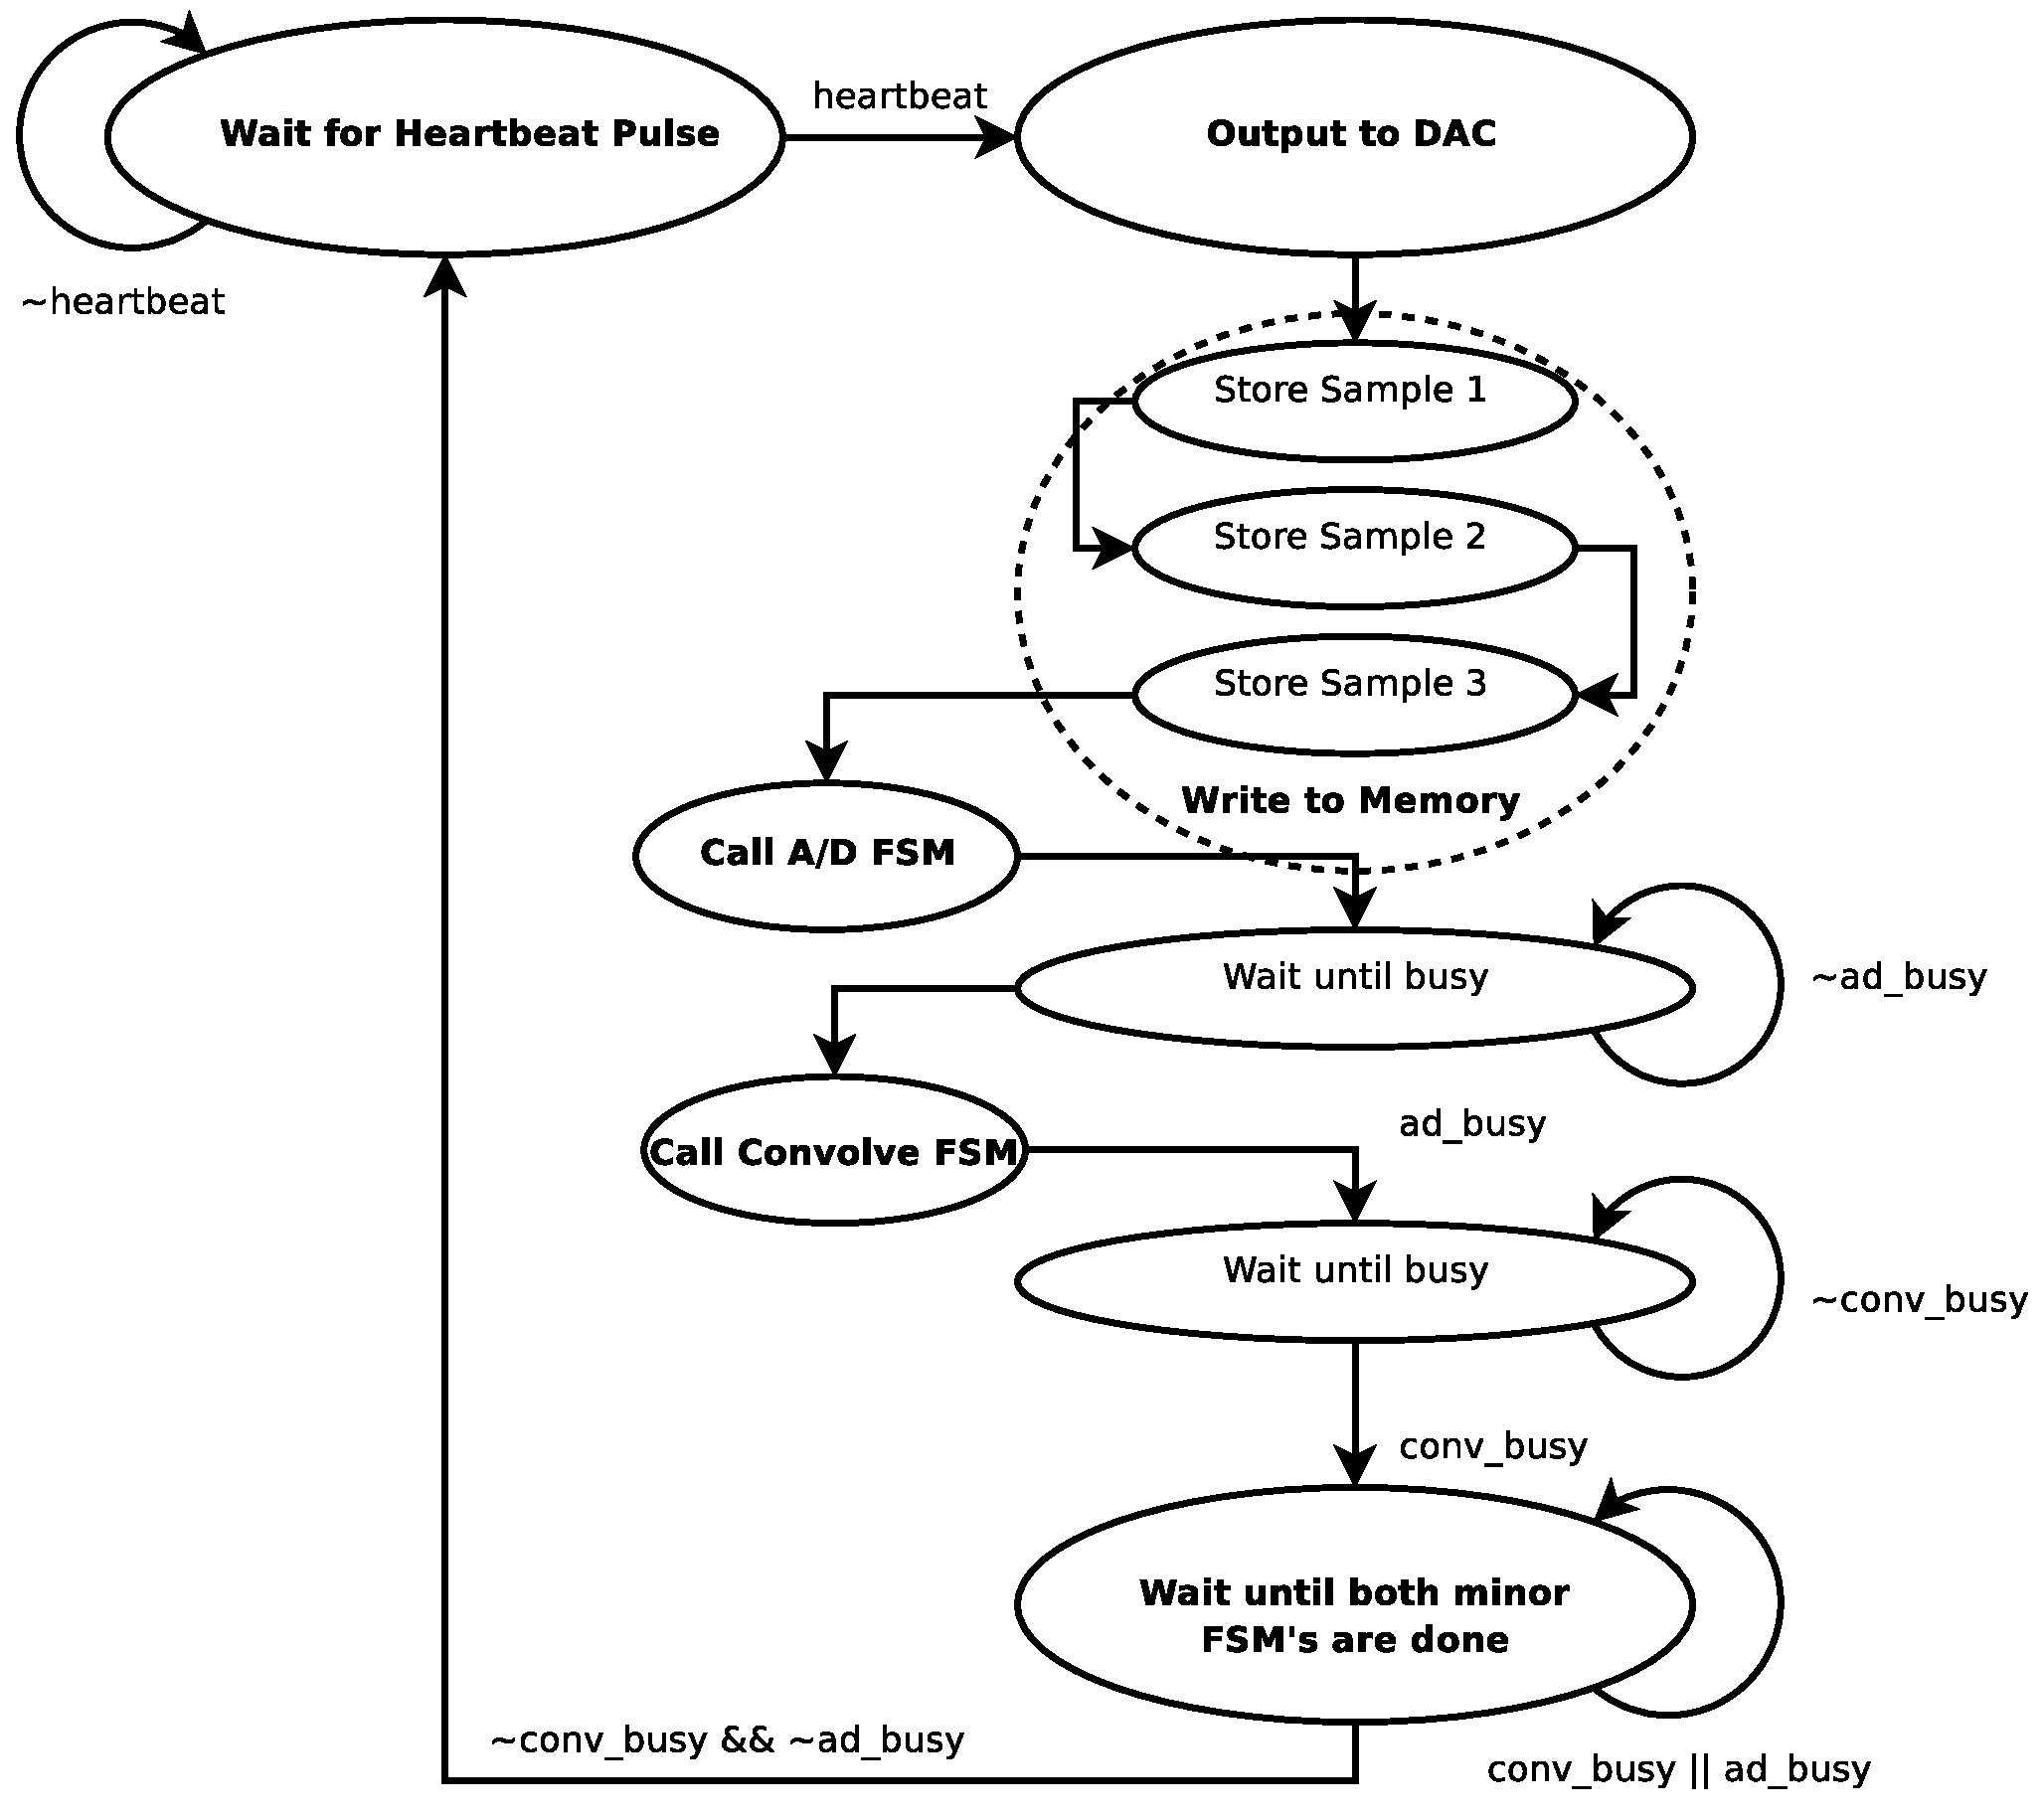
\includegraphics[scale=0.40]{majorfsm.eps}
	\caption{Transition diagram for the major FSM.}
	\label{fig:majorfsm}
	\end{figure}

	The signals the major FSM is responsible for are RAM write enable
	(\texttt{ram\_we}) and D/A chip enable (\texttt{da\_csb}).  Writing to RAM
	takes three clock cycles (hence the three states in the transition
	diagram).  RAM write enable is high for the last two clock cycles of this
	set of states.  Internally, a 4-bit counter is maintained as the pointer to
	the memory location where data should be read or written.  This counter
	effectively makes the RAM a ring buffer.  The counter is incremented at
	each heartbeat pulse (20 khz pulse).  Unless the IO module read signal
	(\texttt{io\_rwb}) is high (only a few clock cycles when the AD minor FSM
	is active), the data bus takes the value of the D/A buffer inside the IO
	module.  The D/A chip latches that value by asserting one of the D/A chip
	enable signals low for one clock cycle (the DAC output state).

	After saving input to memory and writing the output, the major FSM starts
	two minor FSM's.  First it sends a start pulse to the minor FSM responsible
	for sampling.  This pulse is sent during the one cycle Call AD FSM state.
	The next state waits until the minor AD FSM is busy.  When this happens, the
	next state will call the minor convolution FSM.  The next state waits for the
	convolution FSM to start.  When both minor FSM's begin running in parallel,
	the major FSM enters a state where it waits for both minor FSM's to finish.
	At this point, the major FSM goes idle and waits for the heartbeat pulse to
	restart.

		\subsubsection{Convolver FSM}
		This minor FSM is responsible for four control signals: the busy signal
		to the major FSM (\texttt{conv\_busy}), the IO port write enable for
		the D/A buffer (\texttt{dar\_we}), the zero signal to clear the
		accumulator module inside the arithmetic unit (\texttt{fzero}), and the
		accumulate pulse to the accumulator module (\texttt{facc}).  The
		convolver FSM is fairly simple.  State is maintained by a 7-bit
		counter.  Bits 5 through 2 hold the most meaning.  These four bits
		determine the ROM address used in convolution.  The first two bits have
		the effect of making each ROM address valid for four clock cycles.
		This is to ensure that the signals going through the RAM, ROM, and
		arithmetic unit have enough time to propagate through and stabilize.
		The last bit indicates whether convolution is finished or not.
		
		At the end of each four clock cycle state (state[1] and state[0] are
		both one and the finished bit is not high), the \texttt{facc} pulse is
		sent to the accumulator.  The accumulator is zeroed (\texttt{fzero}
		high) at all times except when the FSM is inactive (\texttt{conv\_busy}
		is low).  When convolution is done, the FSM waits a few cycles, then writes
		the result out of the arithmetic unit into the D/A buffer by sending
		the buffer write enable pulse to the IO unit (\texttt{dar\_we}).

		\subsubsection{A/D Controller FSM}
		The process to sample an analog signal and convert it to a digital signal
		goes as follows:  enable the A/D chip, wait for it to finish
		(an operation taking on the order of 10$\mu$s), read the value into the
		IO port A/D buffer.  The A/D chip sends a status signal that is high when
		the chip is busy.  The buffer's contents will be saved in memory at the
		next heartbeat pulse.

		\begin{figure}[ht]
		\centering
		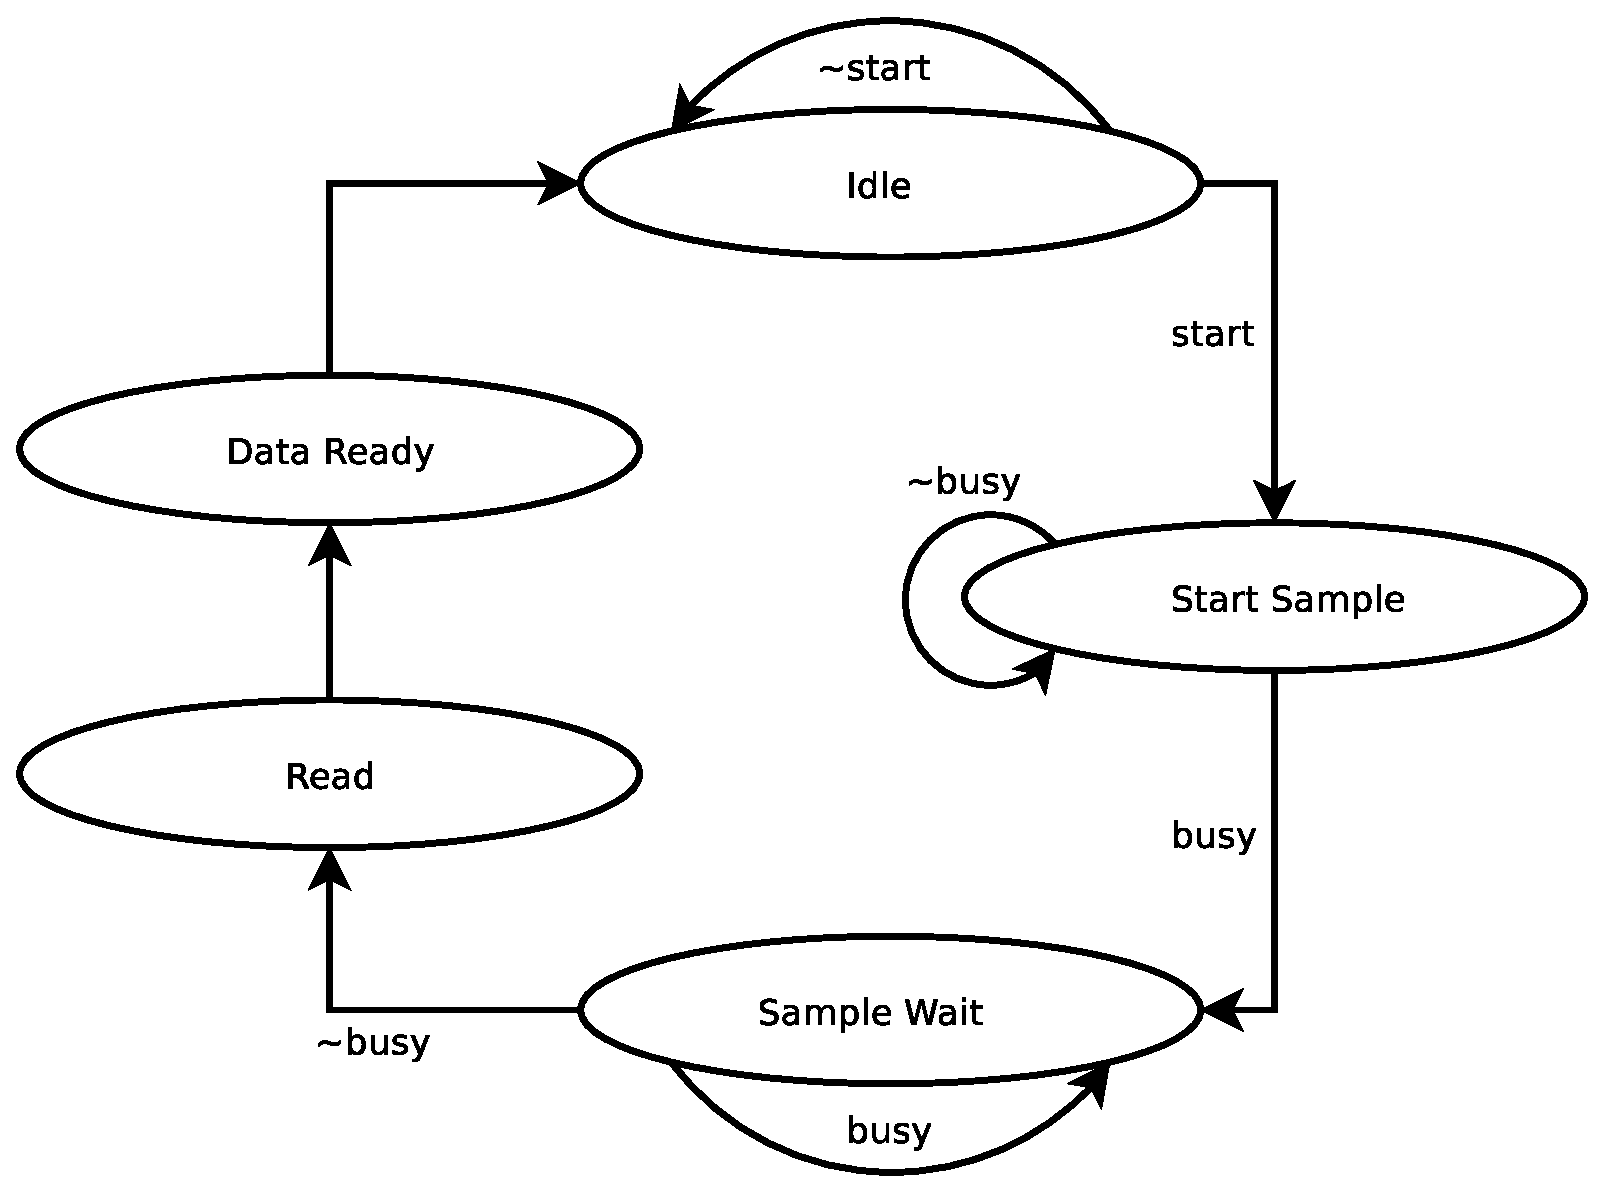
\includegraphics[scale=0.40]{adfsm.eps}
		\caption{Transition diagram for the A/D FSM.}
		\label{fig:adfsm}
		\end{figure}



	\subsection{Arithmetic Unit}
	The outputs of the two memory units are inputs to this module.  The ram input is
	especially notable.  The address of the RAM begin accessed is the subtraction of the
	ROM address from the RAM address stored in the major FSM.  When the convolution FSM
	is not running, the ROM address is zero, and so writing to the RAM is not affected.
	When the convolution FSM is active, the addresses change so that
	convolution can be completed.

	\begin{figure}[ht]
	\centering
	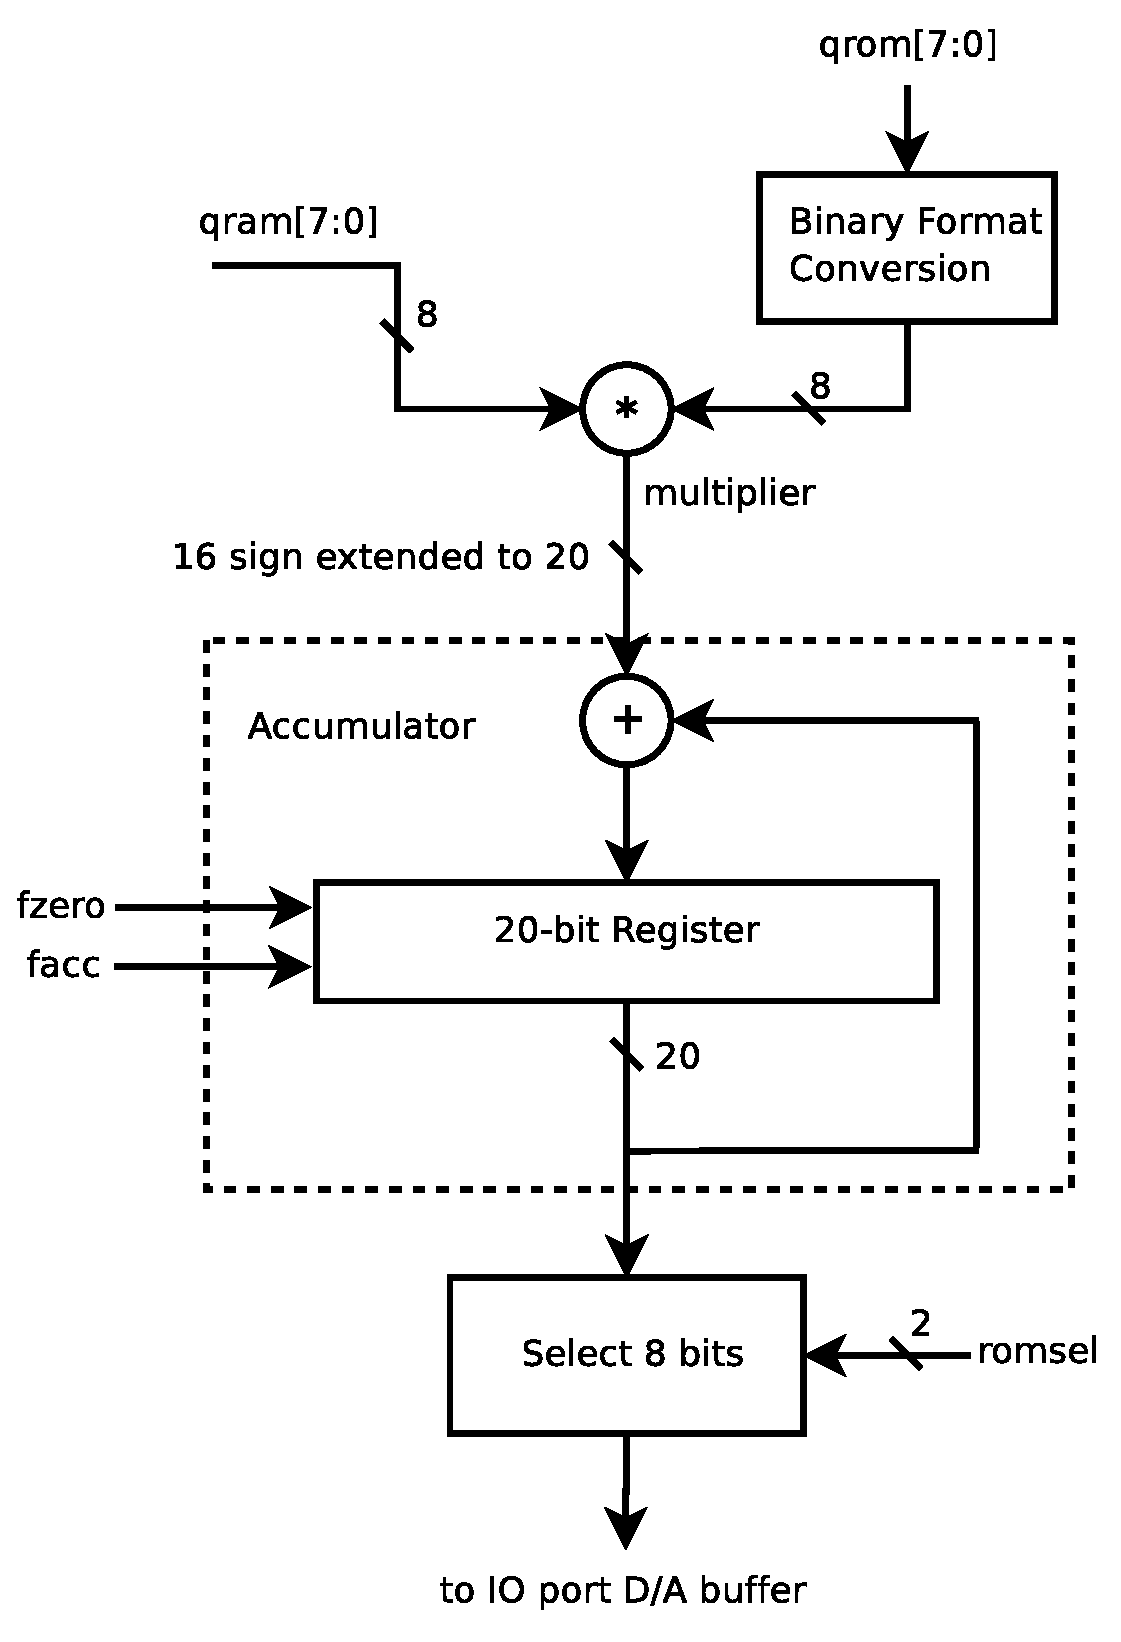
\includegraphics[scale=0.40]{math.eps}
	\caption{Arithmetic unit internals.}
	\label{fig:math}
	\end{figure}

	The arithmetic unit is constructed from a chain of 3 modules: the binary format converter,
	the multiplier, and the accumulator.  The converter and accumulator are discussed below.
	The multiplier is a combinational circuit created using Altera's MegaFunction Wizard.  Figure
	~\ref{fig:math} shows how the three modules are linked together.

		\subsubsection{Sign Multiple to 2's Complement Conversion}
		The multiplier and accumulator produce signed output, so the input to
		those components needed to have 2's complement binary format.  The RAM
		contents were in 2's complement but the ROM output was in sign multiple
		binary format.  For positive numbers, those whose MSB is zero,
		no change is necessary.  For negative values, bits N-1:0 are flipped
		and 1 is added to the resulting number.  This conversion can be done in
		one line of Verilog.

		\subsubsection{Accumulator}
		On every \texttt{facc} pulse, the accumulator adds the value in its internal
		register to the result of the multiplier.
	
\section{Control Signal Timing}

\section{Testing and Debugging}


\section{Conclusions}
	Having two separate stages in this project is key.  The first stage ensures
	that all the wiring is correct.  This makes debugging of the following
	stage much more easy.  The first minor A/D FSM written ended up being much
	more complicated than it needed to be.  When it came time to plug the FSM
	into the full filter, the task was daunting and I rewrote it.


\newpage
\section{Appendix B: FSM Source Code}
	\subsection{Major FSM}
	\begin{lgrind}
	\input majorfsm.v.latex
	\end{lgrind}

	\subsection{AD FSM}
	\begin{lgrind}
	\input adfsm.v.latex
	\end{lgrind}

	\subsection{Convolution FSM}
	\begin{lgrind}
	\input convfsm.v.latex
	\end{lgrind}

\end{document}
